\documentclass{standalone}
\usepackage{tikz}
\usetikzlibrary{patterns, positioning}

\begin{document}
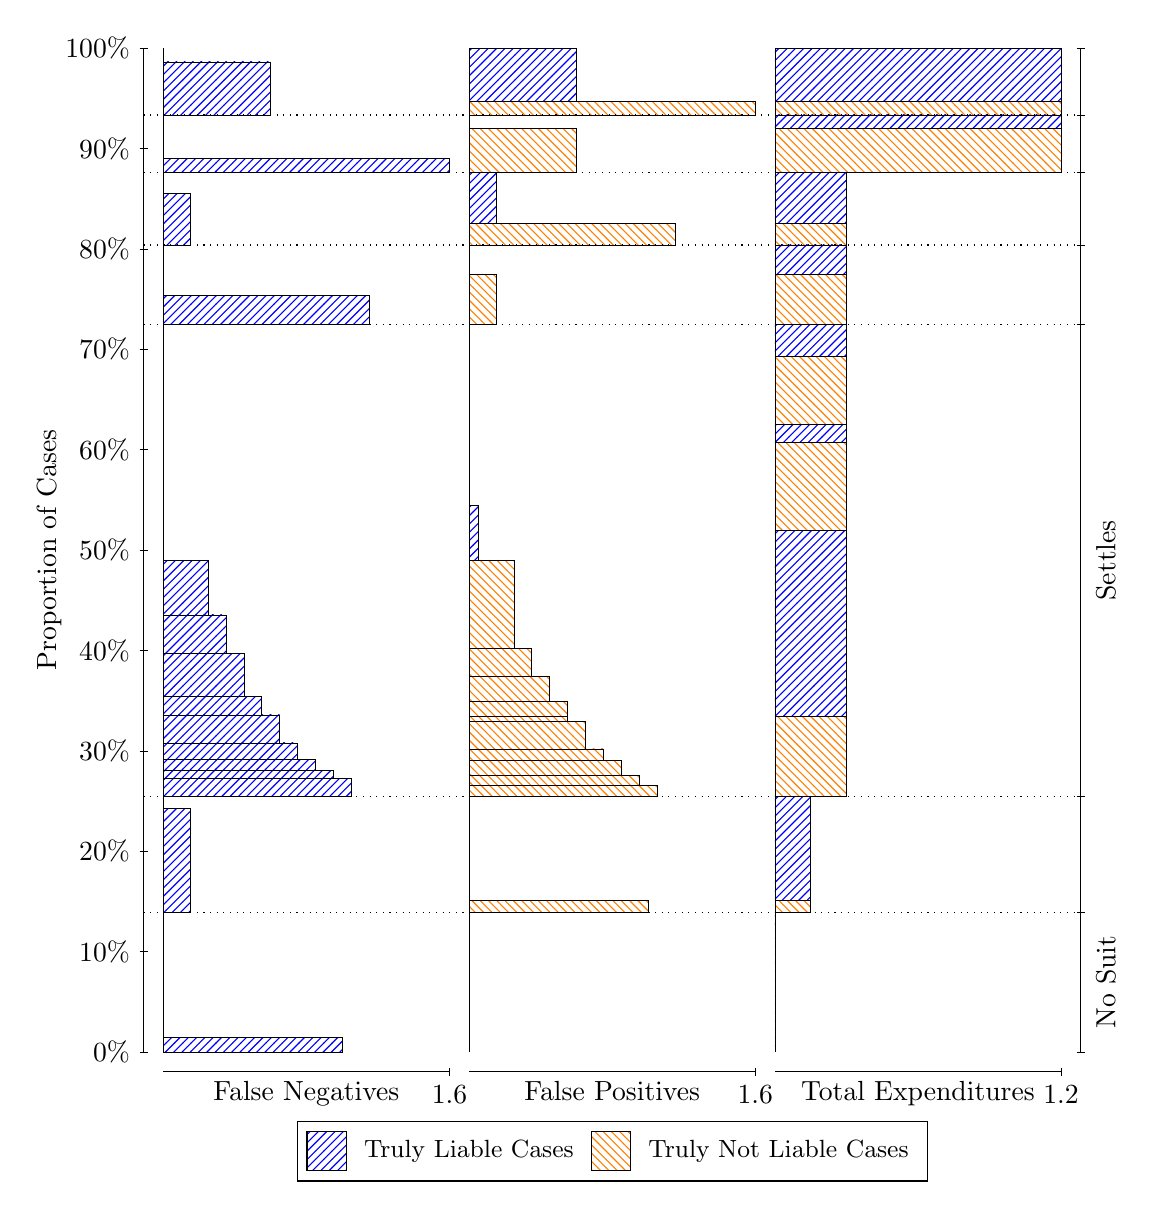
\begin{tikzpicture}
\draw[black, very thin] (1.5,1.75) -- (1.5,14.5);
\node[rotate=90, anchor=center] at (0.3, 8.125) {Proportion of Cases};
\draw[black, very thin] (1.45,1.75) -- (1.55,1.75);
\node[anchor=east] at (1.45, 1.75) {0\%};
\draw[black, very thin] (1.45,3.025) -- (1.55,3.025);
\node[anchor=east] at (1.45, 3.025) {10\%};
\draw[black, very thin] (1.45,4.3) -- (1.55,4.3);
\node[anchor=east] at (1.45, 4.3) {20\%};
\draw[black, very thin] (1.45,5.575) -- (1.55,5.575);
\node[anchor=east] at (1.45, 5.575) {30\%};
\draw[black, very thin] (1.45,6.85) -- (1.55,6.85);
\node[anchor=east] at (1.45, 6.85) {40\%};
\draw[black, very thin] (1.45,8.125) -- (1.55,8.125);
\node[anchor=east] at (1.45, 8.125) {50\%};
\draw[black, very thin] (1.45,9.4) -- (1.55,9.4);
\node[anchor=east] at (1.45, 9.4) {60\%};
\draw[black, very thin] (1.45,10.675) -- (1.55,10.675);
\node[anchor=east] at (1.45, 10.675) {70\%};
\draw[black, very thin] (1.45,11.95) -- (1.55,11.95);
\node[anchor=east] at (1.45, 11.95) {80\%};
\draw[black, very thin] (1.45,13.225) -- (1.55,13.225);
\node[anchor=east] at (1.45, 13.225) {90\%};
\draw[black, very thin] (1.45,14.5) -- (1.55,14.5);
\node[anchor=east] at (1.45, 14.5) {100\%};

\draw[black, very thin] (13.4,1.75) -- (13.4,14.5);
\draw[black, very thin] (13.35,1.75) -- (13.45,1.75);
\node[anchor=west] at (13.35, 1.75) {};
\draw[black, very thin] (13.35,3.524) -- (13.45,3.524);
\node[anchor=west] at (13.35, 3.524) {};
\draw[black, very thin] (13.35,4.9969) -- (13.45,4.9969);
\node[anchor=west] at (13.35, 4.9969) {};
\draw[black, very thin] (13.35,10.99) -- (13.45,10.99);
\node[anchor=west] at (13.35, 10.99) {};
\draw[black, very thin] (13.35,11.999) -- (13.45,11.999);
\node[anchor=west] at (13.35, 11.999) {};
\draw[black, very thin] (13.35,12.922) -- (13.45,12.922);
\node[anchor=west] at (13.35, 12.922) {};
\draw[black, very thin] (13.35,13.65) -- (13.45,13.65);
\node[anchor=west] at (13.35, 13.65) {};
\draw[black, very thin] (13.35,14.5) -- (13.45,14.5);
\node[anchor=west] at (13.35, 14.5) {};

\draw[black, very thin, pattern color=blue, pattern=north east lines] (1.75,1.75) rectangle (4.0208,1.9366);
\draw[black, very thin, pattern color=orange, pattern=north west lines] (1.75,1.9366) rectangle (1.75,3.524);
\draw[black, very thin, pattern color=blue, pattern=north east lines] (1.75,3.524) rectangle (2.0906,4.8451);
\draw[black, very thin, pattern color=orange, pattern=north west lines] (1.75,4.8451) rectangle (1.75,4.9969);
\draw[black, very thin, pattern color=blue, pattern=north east lines] (1.75,4.9969) rectangle (4.1344,5.2208);
\draw[black, very thin, pattern color=blue, pattern=north east lines] (1.75,5.2208) rectangle (3.9073,5.3238);
\draw[black, very thin, pattern color=blue, pattern=north east lines] (1.75,5.3238) rectangle (3.6802,5.4654);
\draw[black, very thin, pattern color=blue, pattern=north east lines] (1.75,5.4654) rectangle (3.4531,5.6748);
\draw[black, very thin, pattern color=blue, pattern=north east lines] (1.75,5.6748) rectangle (3.226,6.0296);
\draw[black, very thin, pattern color=blue, pattern=north east lines] (1.75,6.0296) rectangle (2.999,6.2627);
\draw[black, very thin, pattern color=blue, pattern=north east lines] (1.75,6.2627) rectangle (2.7719,6.8074);
\draw[black, very thin, pattern color=blue, pattern=north east lines] (1.75,6.8074) rectangle (2.5448,7.2996);
\draw[black, very thin, pattern color=blue, pattern=north east lines] (1.75,7.2996) rectangle (2.3177,7.9932);
\draw[black, very thin, pattern color=orange, pattern=north west lines] (1.75,7.9932) rectangle (1.75,10.99);
\draw[black, very thin, pattern color=blue, pattern=north east lines] (1.75,10.99) rectangle (4.3615,11.361);
\draw[black, very thin, pattern color=orange, pattern=north west lines] (1.75,11.361) rectangle (1.75,11.999);
\draw[black, very thin, pattern color=blue, pattern=north east lines] (1.75,11.999) rectangle (2.0906,12.651);
\draw[black, very thin, pattern color=orange, pattern=north west lines] (1.75,12.651) rectangle (1.75,12.922);
\draw[black, very thin, pattern color=blue, pattern=north east lines] (1.75,12.922) rectangle (5.3833,13.097);
\draw[black, very thin, pattern color=orange, pattern=north west lines] (1.75,13.097) rectangle (1.75,13.65);
\draw[black, very thin, pattern color=blue, pattern=north east lines] (1.75,13.65) rectangle (3.1125,14.324);
\draw[black, very thin, pattern color=orange, pattern=north west lines] (1.75,14.324) rectangle (1.75,14.5);
\draw[black, very thin, pattern color=orange, pattern=north west lines] (5.6333,1.75) rectangle (5.6333,3.3373);
\draw[black, very thin, pattern color=blue, pattern=north east lines] (5.6333,3.3373) rectangle (5.6333,3.524);
\draw[black, very thin, pattern color=orange, pattern=north west lines] (5.6333,3.524) rectangle (7.9042,3.6758);
\draw[black, very thin, pattern color=blue, pattern=north east lines] (5.6333,3.6758) rectangle (5.6333,4.9969);
\draw[black, very thin, pattern color=orange, pattern=north west lines] (5.6333,4.9969) rectangle (8.0177,5.1325);
\draw[black, very thin, pattern color=orange, pattern=north west lines] (5.6333,5.1325) rectangle (7.7906,5.2614);
\draw[black, very thin, pattern color=orange, pattern=north west lines] (5.6333,5.2614) rectangle (7.5635,5.4487);
\draw[black, very thin, pattern color=orange, pattern=north west lines] (5.6333,5.4487) rectangle (7.3365,5.6001);
\draw[black, very thin, pattern color=orange, pattern=north west lines] (5.6333,5.6001) rectangle (7.1094,5.9448);
\draw[black, very thin, pattern color=orange, pattern=north west lines] (5.6333,5.9448) rectangle (6.8823,6.0121);
\draw[black, very thin, pattern color=orange, pattern=north west lines] (5.6333,6.0121) rectangle (6.8823,6.203);
\draw[black, very thin, pattern color=orange, pattern=north west lines] (5.6333,6.203) rectangle (6.6552,6.5151);
\draw[black, very thin, pattern color=orange, pattern=north west lines] (5.6333,6.5151) rectangle (6.4281,6.8725);
\draw[black, very thin, pattern color=orange, pattern=north west lines] (5.6333,6.8725) rectangle (6.201,7.994);
\draw[black, very thin, pattern color=blue, pattern=north east lines] (5.6333,7.994) rectangle (5.7469,8.6876);
\draw[black, very thin, pattern color=blue, pattern=north east lines] (5.6333,8.6876) rectangle (5.6333,10.99);
\draw[black, very thin, pattern color=orange, pattern=north west lines] (5.6333,10.99) rectangle (5.974,11.629);
\draw[black, very thin, pattern color=blue, pattern=north east lines] (5.6333,11.629) rectangle (5.6333,11.999);
\draw[black, very thin, pattern color=orange, pattern=north west lines] (5.6333,11.999) rectangle (8.2448,12.27);
\draw[black, very thin, pattern color=blue, pattern=north east lines] (5.6333,12.27) rectangle (5.974,12.922);
\draw[black, very thin, pattern color=orange, pattern=north west lines] (5.6333,12.922) rectangle (6.9958,13.475);
\draw[black, very thin, pattern color=blue, pattern=north east lines] (5.6333,13.475) rectangle (5.6333,13.65);
\draw[black, very thin, pattern color=orange, pattern=north west lines] (5.6333,13.65) rectangle (9.2667,13.827);
\draw[black, very thin, pattern color=blue, pattern=north east lines] (5.6333,13.827) rectangle (6.9958,14.5);
\draw[black, very thin, pattern color=orange, pattern=north west lines] (9.5167,1.75) rectangle (9.5167,3.3373);
\draw[black, very thin, pattern color=blue, pattern=north east lines] (9.5167,3.3373) rectangle (9.5167,3.524);
\draw[black, very thin, pattern color=orange, pattern=north west lines] (9.5167,3.524) rectangle (9.9708,3.6758);
\draw[black, very thin, pattern color=blue, pattern=north east lines] (9.5167,3.6758) rectangle (9.9708,4.9969);
\draw[black, very thin, pattern color=orange, pattern=north west lines] (9.5167,4.9969) rectangle (10.425,6.0121);
\draw[black, very thin, pattern color=blue, pattern=north east lines] (9.5167,6.0121) rectangle (10.425,8.3746);
\draw[black, very thin, pattern color=orange, pattern=north west lines] (9.5167,8.3746) rectangle (10.425,9.4961);
\draw[black, very thin, pattern color=blue, pattern=north east lines] (9.5167,9.4961) rectangle (10.425,9.7201);
\draw[black, very thin, pattern color=orange, pattern=north west lines] (9.5167,9.7201) rectangle (10.425,10.581);
\draw[black, very thin, pattern color=blue, pattern=north east lines] (9.5167,10.581) rectangle (10.425,10.99);
\draw[black, very thin, pattern color=orange, pattern=north west lines] (9.5167,10.99) rectangle (10.425,11.629);
\draw[black, very thin, pattern color=blue, pattern=north east lines] (9.5167,11.629) rectangle (10.425,11.999);
\draw[black, very thin, pattern color=orange, pattern=north west lines] (9.5167,11.999) rectangle (10.425,12.27);
\draw[black, very thin, pattern color=blue, pattern=north east lines] (9.5167,12.27) rectangle (10.425,12.922);
\draw[black, very thin, pattern color=orange, pattern=north west lines] (9.5167,12.922) rectangle (13.15,13.475);
\draw[black, very thin, pattern color=blue, pattern=north east lines] (9.5167,13.475) rectangle (13.15,13.65);
\draw[black, very thin, pattern color=orange, pattern=north west lines] (9.5167,13.65) rectangle (13.15,13.827);
\draw[black, very thin, pattern color=blue, pattern=north east lines] (9.5167,13.827) rectangle (13.15,14.5);
\draw[black, dotted] (1.5,3.524) -- (13.4,3.524);
\draw[black, dotted] (1.5,4.9969) -- (13.4,4.9969);
\draw[black, dotted] (1.5,10.99) -- (13.4,10.99);
\draw[black, dotted] (1.5,11.999) -- (13.4,11.999);
\draw[black, dotted] (1.5,12.922) -- (13.4,12.922);
\draw[black, dotted] (1.5,13.65) -- (13.4,13.65);
\draw[black, very thin] (1.75,1.5) -- (5.3833,1.5);
\node[anchor=north] at (3.5667, 1.5) {False Negatives};
\draw[black, very thin] (5.3833,1.45) -- (5.3833,1.55);
\node[anchor=north] at (5.3833, 1.45) {1.6};

\draw[black, very thin] (5.6333,1.5) -- (9.2667,1.5);
\node[anchor=north] at (7.45, 1.5) {False Positives};
\draw[black, very thin] (9.2667,1.45) -- (9.2667,1.55);
\node[anchor=north] at (9.2667, 1.45) {1.6};

\draw[black, very thin] (9.5167,1.5) -- (13.15,1.5);
\node[anchor=north] at (11.333, 1.5) {Total Expenditures};
\draw[black, very thin] (13.15,1.45) -- (13.15,1.55);
\node[anchor=north] at (13.15, 1.45) {1.2};

\node[black, centered, rotate=90] at (13.72, 2.637) {No Suit};

\node[black, centered, rotate=90] at (13.72, 7.9936) {Settles};





\draw (7.449999999999999,1.5) node[draw=none] (baseCoordinate) {};
\begin{scope}[align=center]
        \matrix[scale=0.5, draw=black, below=0.5cm of baseCoordinate, nodes={draw}, column sep=0.1cm]{
            \node[rectangle, draw, minimum width=0.5cm, minimum height=0.5cm, pattern=north east lines, pattern color=blue] {}; &
            \node[draw=none, font=\small] (B) {Truly Liable Cases}; &
            \node[rectangle, draw, minimum width=0.5cm, minimum height=0.5cm, pattern=north west lines, pattern color=orange] {}; &
            \node[draw=none, font=\small] (B) {Truly Not Liable Cases}; \\
            };
\end{scope}

\end{tikzpicture}
\end{document}